\documentclass{article}

%Header Dimensions
%https://tex.stackexchange.com/questions/40183/problem-with-the-header-footer-width#40184
\usepackage[margin=0.5in,bottom=0.5in,top=0.5in]{geometry}

%Package required for empty set
\usepackage{amssymb}

%Package required for Comb/Perm symbol and matrices
\usepackage{amsmath}

%Package for graphics
\usepackage{graphicx}

%Package for placing graphics
\usepackage{float}

%Places box around graphics
% Uncomment to box 
% \floatstyle{boxed} 
% \restylefloat{figure}


%For inserting code
\usepackage{listings}
%https://www.sharelatex.com/learn/Code_listing

\begin{document}

	
%%%%%%%%%%%%%%%%%
%CUSTOM COMMANDS%
%%%%%%%%%%%%%%%%%

	%This line surpresses the page number
%https://tex.stackexchange.com/questions/7355/how-to-suppress-page-number
\thispagestyle{empty}

%Make empty set pretty
% https://tex.stackexchange.com/questions/22798/nice-looking-empty-setup
\let\oldemptyset\emptyset
\let\emptyset\varnothing


%Combinatorial notation
%From https://tex.stackexchange.com/questions/107125/is-there-a-command-to-write-the-form-of-a-combination-or-permutation
\newcommand*{\Perm}[2]{{}^{#1}\!P_{#2}}
\newcommand*{\Comb}[2]{{}_{#1}C_{#2}}


	
\textbf{	Matt Fletcher CS317-02 Homework 1}
\smallskip

1. 

\begin{figure}[H]

  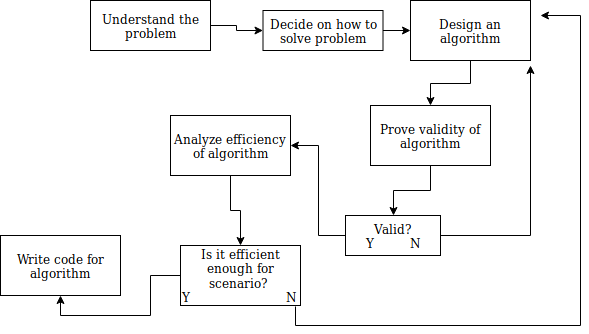
\includegraphics[scale=0.78]{P2Flowchart}
  \caption{Flowchart for design of algorithm}
\end{figure}


\noindent\rule{8cm}{0.4pt}

2. An example of a non-basic operation is something that will not count significantly towards the runtime of the program as input size $n$ increases. These include operations such as print statements, variable declarations, etc. 

A basic operation is something that contributes significantly to the runtime of the program. This could be as simple as a comparison in a while loop:

\begin{lstlisting}
	int n = 0; //non-basic
	do{
		cout << "Hey" << endl; //non-basic
		n++; //basic
	}while(n<value) //basic
\end{lstlisting}

In the above code, the lines of code are commented with their basic-ness. Even though the incrementing and the while loop are both considered basic operations, the coefficient drops out when input size $n$ increases, therefore, it does not matter which one is chosen as a basic step. 

\noindent\rule{8cm}{0.4pt}

3. $\log (n), n, n\log (n), n^2, n^3, 2^n, n\!$

\noindent\rule{8cm}{0.4pt}


4.1.

a. $\Omega(n)$, in the event that the desired search term is not in the list. 
	
b. O(1), in the event that the desired search term is in index 0. 

c. $\Theta(n)$ best represents the average case. 

\noindent\rule{2cm}{0.4pt}

4.2.

a) True

b) True

c) False

d) False


\noindent\rule{8cm}{0.4pt}

5. The three asymptotic notations:

$O(n)$ (aka big O notation) represents the upper bound of the efficiency of the algorithm.

$\Omega(n)$ (aka big Omega notation) represents the lower bound of the efficiency of the algorithm. 

$\Theta(n)$ (aka big theta notation) represents an equal efficiency of the algorithm. 


TODO add example

\noindent\rule{8cm}{0.4pt}


6.  $\log (n), n, n\log (n), n^2, n^3, 2^n, n\!$

	Logarithmic, linear, linarithmic, quadratic, cubic, exponential, factorial. 

\noindent\rule{8cm}{0.4pt}

7.  

To analyze a non-recursive algorithm:

Decide on a parameter indicating input size. 

Find the major significant steps in the program. Steps such as initializing variables are not significant. Steps that are done on each iteration of the algorithm (such as a comparison) are. The goal is to find the step that most significantly effects the performance of the algorithm. 

Set up a sum expressing how many times this step is run. 

Find a closed form solution for the sum, or calculate its growth rate. 

\noindent\rule{8cm}{0.4pt}


8. 

Decide on a parameter indicating input size. 

Identify the algorithms basic operation. 

Check if the execution count varies on different input sizes. 

Set up a recurrence relation with an appropriate base condition for the number of times the basic operation is executed. 

Solve the recurrence for a closed form. 


\noindent\rule{8cm}{0.4pt}


9. 

MYSTERY

a. This algorithm calculates the sum of squares up to and including some input $n$. 

b. The basic operation is $S \leftarrow S + i\cdot i$

c. The basic operation is computed $n$ times. 

d. This algorithm operates in a linear efficiency.

\noindent\rule{2cm}{0.4pt}

SECRET

a. This algorithm calculates the difference between the maximum and minimum values in an array of numbers. 

b. The basic operation is either one of the comparisons. 

c. For each iteration (of which there are n-1 of), there are 2 comparisons made. This means that the number of comparisons is $2(n-1)$, which asymptotically rises to show that this operates in a linear efficiency. 

\noindent\rule{2cm}{0.4pt}

ENIGMA

a. This algorithm checks if a 2D matrix is symmetrical about the diagonal axis. 

b. The basic operation is $if A[i,j] \neq A[j,i]$. 

c. The outer loop operates $n-1$ times, and the inner loop operates between $n-2$ and $1$ times. 

d.  Because this happens inside two nested loops with approximately equal asymptotic sizes, this means that the comparison happens approximately $n^2$ times. Therefore, this operates in quadratic efficiency. 


\noindent\rule{8cm}{0.4pt}


10. 

\begin{lstlisting}
	def factorial(n):
		if(n==1):
			return 1
		else:
			return n*factorial(n-1)
\end{lstlisting}

The basic operation is the multiplication in the bottom line. 

Let $M(n)$ represent the number of multiplications done. 

$M(n) = M(n-1) + 1$

The base case is when no multiplications are done with $n=0$. Therefore, $M(0) = 0$. 

Use a backward substitution:

\[M(n) = M(n-1) + 1\]

\[M(n) = M(n-2) + 1 + 1\]

\[M(n) = M(n-3) + 1 + 1 + 1\]


A pattern is apparent: 

\[M(n) = M(0) + n\]


As the base case has $M(0) = 0$, this simplifies to: 

\[\boxed{M(n) \in \Theta(n)}\]


\noindent\rule{8cm}{0.4pt}


11. 

\begin{lstlisting}
	ALGORITHM: FIND IN PHONEBOOK

	//Assume phonebook has names listed in alphabetic order with no duplicates
	//Assume n names are in book
	//Assume name to be found is called "guess"

	//Declare pointers to the following indexed entries
	left = 0
	right = n-1
	middle = ceil(n/2)

	*****

	if guess == middle:
		return guess
	fi

	if guess < middle:
		right = middle
		middle = ceil(right/2)
		GOTO *****
	fi


	if guess > middle:
		left = middle
		middle = ceil(left/2)
		GOTO *****
	fi

\end{lstlisting}

The worst case is where the node to be found is at the beginning or the end of the list. 

Because the algorithm halves the search space each time it runs, the algorithm runs in $O(\log n)$. 

\noindent\rule{8cm}{0.4pt}


12. 

\begin{lstlisting}
	ALGORITHM: CHECK IF SORTED

	for item in list(0,i-1):
		if item[i] >  item[i+1] then
			return false
		fi
	return true
\end{lstlisting}

The worst case scenario in this instance is having the last 2 items be out of order. This means that in a list of length $n$, the program must do $n-1$ comparisons. 

Let $C(n)$ represent the number of times the basic operation is executed. 

\[ C(n) = \sum_{i=1}^{n-1} 1 = n-1 \]


\[ n-1 \in \Theta(n)  \]

The time efficiency is $\Theta(n)$


\noindent\rule{8cm}{0.4pt}



13. 

\begin{lstlisting}
	ALGORITHM INSERTION SORT
	i = 1
	while i < size:
		j=1
		while j>0 and A[j-1]>A[j]
			swap A[j] and A[j-1]
			j- - 
		elihw
		i++
	elihw
\end{lstlisting}

TODO ANALYZE

\noindent\rule{8cm}{0.4pt}


14. I do not use an IDE to develop my code. However, Linux has a command line tool called gdb (Gnu DeBugger) that I can use in the same way. 


\begin{figure}[H]

  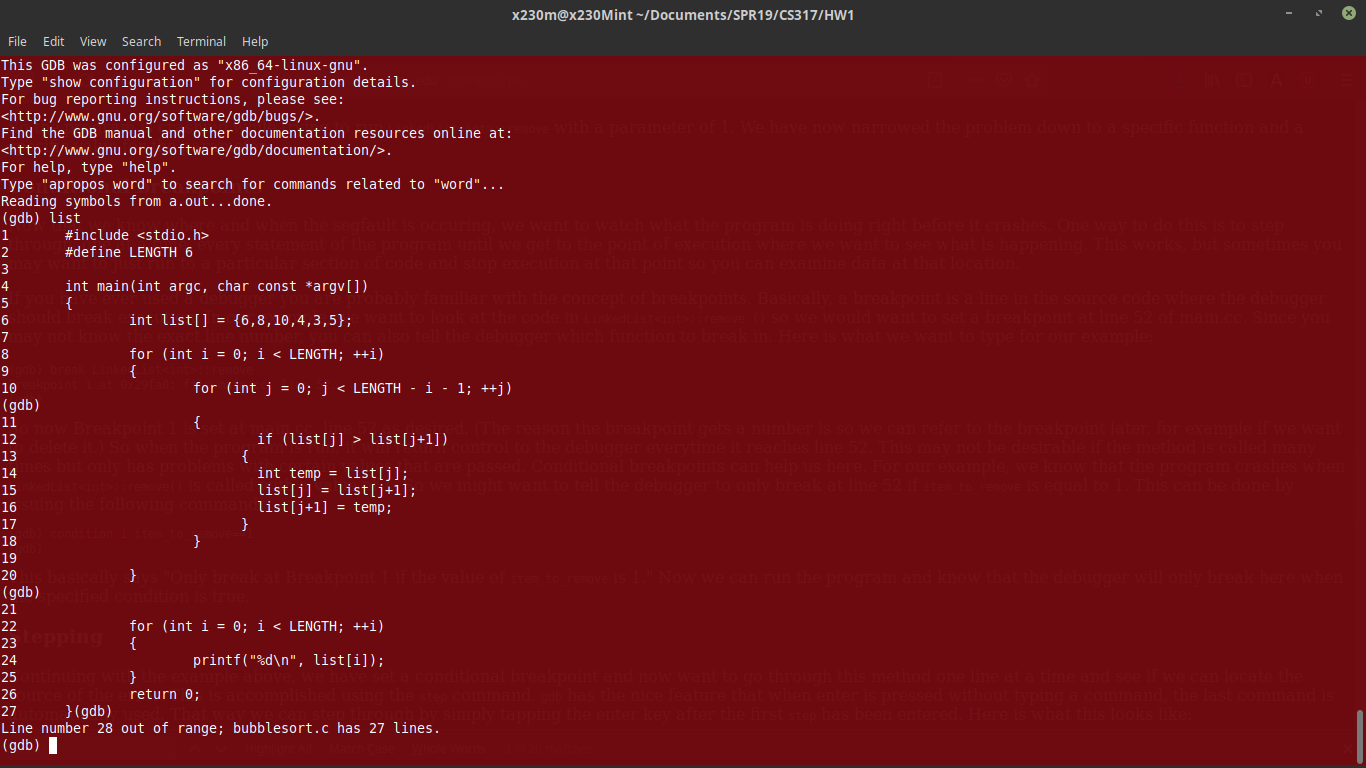
\includegraphics[scale=0.4]{P15-1}
  \caption{Screenshot of debugger tool showing code.}
\end{figure}



\begin{figure}[H]

  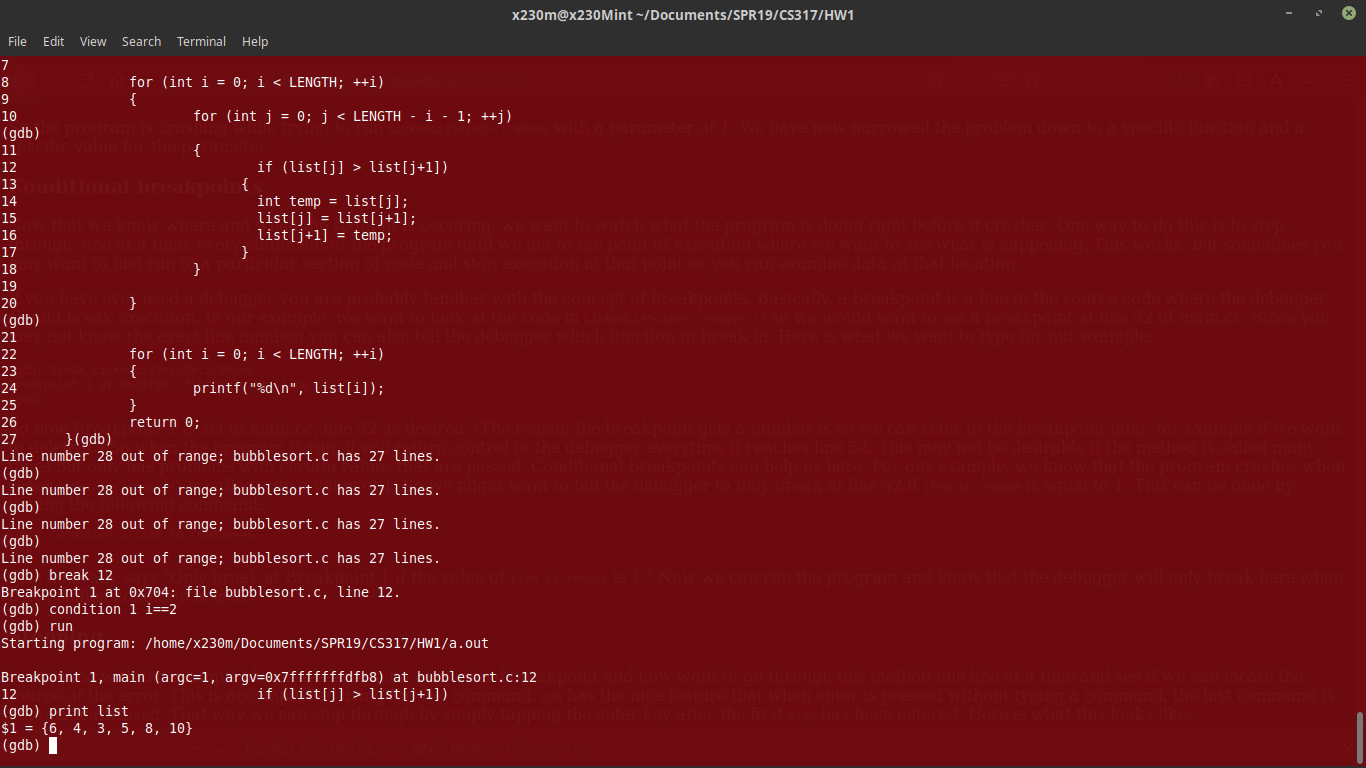
\includegraphics[scale=0.4]{P15-2}
  \caption{A breakpoint has been added, and the list has been printed in its current state. }
\end{figure}



\begin{figure}[H]

  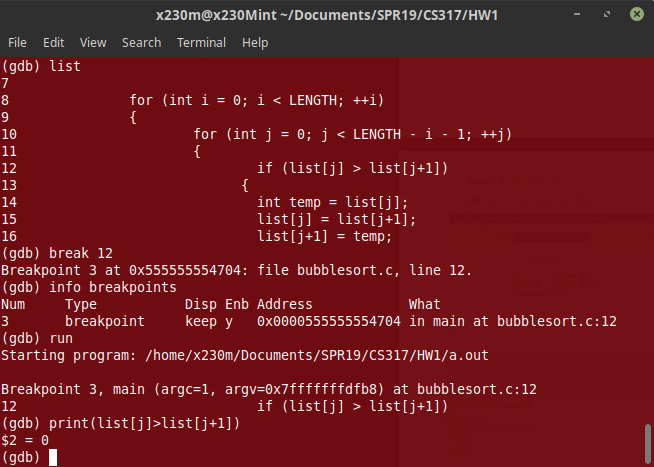
\includegraphics[scale=0.7]{P15-3}
  \caption{Showing that a breakpoint has been added at the given point in the code, and the comparison value is false.}
\end{figure}



\begin{figure}[H]

  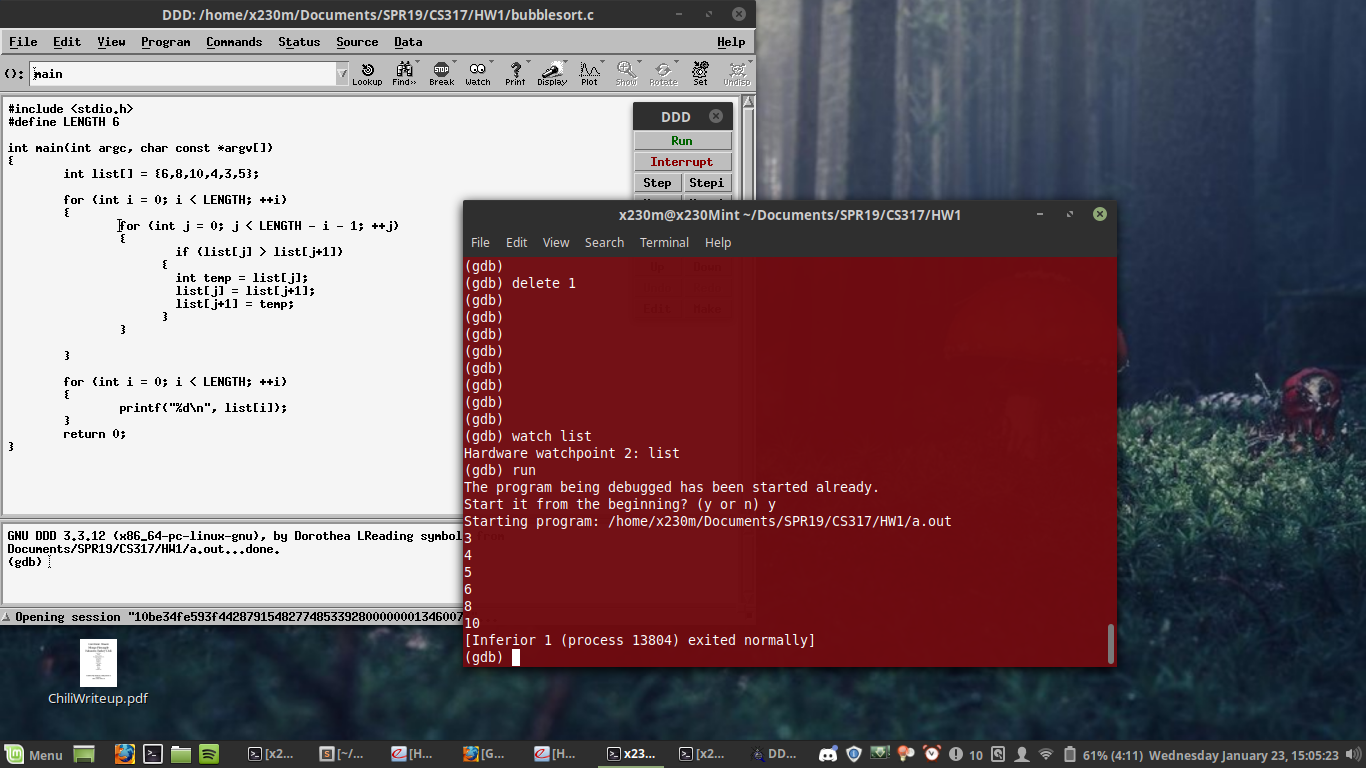
\includegraphics[scale=0.4]{P15-full}
  \caption{The GUI for this program showing the code and the watchpoints. }
\end{figure}



\noindent\rule{8cm}{0.4pt}


15. 

The code is attached in file bruteforce.py. 



\begin{table}[H]
\begin{tabular}{|l|l|}
\hline
Length & Run Time (seconds) \\ \hline
1 & 3.7E-5 \\ \hline
2 & 1.44E-3 \\ \hline
3 & 5.38E-2 \\ \hline
4 & 1.83E0 \\ \hline
5 & 5.91E1 \\ \hline
6 & 1.53E3 \\ \hline
7 & 3.98E4 \\ \hline
\end{tabular}
\end{table}

Calculating the 7 character combinations took approximately 11 hours to run.

I would have run it longer, however, I calculated that at the current rate of growth, calculating every possible 35 character password would have taken past the heat death of the universe to calculate. 

As I assume that an extension of $10^{35}$ years would not be acceptable, I decided to simply truncate the table. 



\noindent\rule{8cm}{0.4pt}



\end{document}